\chapter{Anleitung für Docker starten}
\section{Docker starten}
\begin{enumerate}
    \item Verbinden mit HPC 
    \item Unter \textit{/mnt/data/outside-data/} Ordner mit Namen Projekt anlegen für Studierenden (\textit{mkdir \textless Projektname\textgreater})
    \item Studierenden privaten Key vom Nutzer \textit{docker\_user} geben
    \item Studierende kopiert Daten auf \textit{/mnt/data/outside-data/} $\rightarrow$ die folgenden Schritte beziehen sich auf ein Windows Betriebssystem, für Linuxsysteme sind die ähnlichen Schritte nur die Berechtigungsschritte werden per \textit{chown 700 \textless user\textgreater \textless key\textgreater}
    
    \begin{enumerate}
        \item Studierende speichert Private Key auf PC ab
        \item Verbindung des PCs mit Mosbach VPN (Lehre Netz)
        \item Rechtsklick auf private Key im File Explorer $\rightarrow$ Properties $\rightarrow$ Sicherheit $\rightarrow$ erweitert $\rightarrow$ sollte Berechtigung sehen wie in \autoref{fig:berecht_1}
        \item klicken auf Vererbung Deaktivieren
        \item Hinzufügen klicken $\rightarrow$ SYSTEM suchen $\rightarrow$ Lese- und Execute und Schreibrechte geben $\rightarrow$ Ok klicken
        \item Hinzufügen klicken $\rightarrow$ \textless eigenen Nutzer\textgreater  suchen $\rightarrow$ Lese- und Execute und Schreibrechte geben $\rightarrow$ Ok klicken
        \item Danach sollte Berechtigung aussehen wie in \autoref{fig:berecht_2}
        \item Kommandozeile öffnen $\rightarrow$ wechseln in Directory wo Key legt
        \item Folgendes Kommando eingeben (alles eine Zeile)
        \begin{verbatim}
            scp -i <keyfile Name> -P 2022 <Pfad zu Datenablage>
            docker_user@193.197.11.229:/mnt/data/outside-data/<Name des Projektes>/  
        \end{verbatim}
        \item Information: \textless Pfad zu Datenablage\textgreater ist der Pfad zur Base Directory $\rightarrow$ alles darin wird rüberkopiert / \textless Name des Projektes\textgreater ist ein vorher angelegter Ordner, der den Namen des Projektes trägt, Password eingeben $\rightarrow$ wird von Herrn Müller übergeben
    \end{enumerate}
    \item Dockercontainer installieren $\rightarrow$ wenn Yolov5 bitte unten den Anweisungen folgen
    \item Client schließen und laufen lassen
\end{enumerate}

\begin{figure}
    \centering
    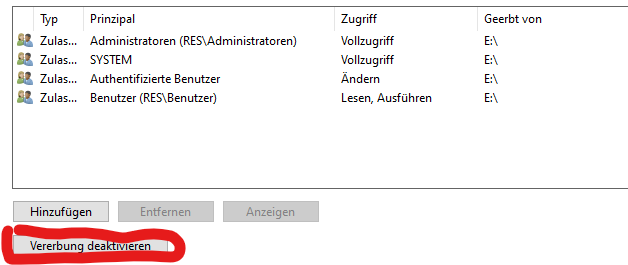
\includegraphics[width=8cm]{data/img/berechtigungen_1.png}
    \caption{Berechtigungen wie sie meistens voreingestellt sind durch Windows}
    \label{fig:berecht_1}
\end{figure}
\begin{figure}
    \centering
    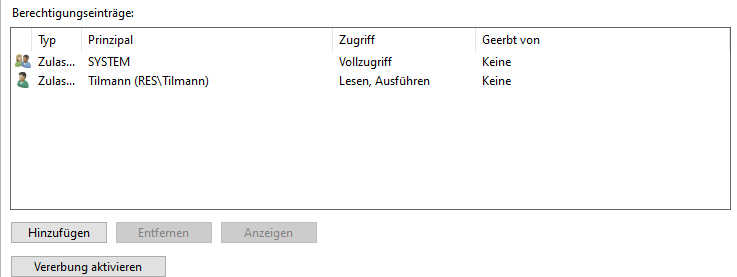
\includegraphics[width=8cm]{data/img/berechtigungen_2.png}
    \caption{Zielzustand Berechtigungen}
    \label{fig:berecht_2}
\end{figure}

\textbf{DIE FOLGENDEN SCHRITTE BEZIEHEN SICH AUSSCHLIEßLICH AUF YOLOv5}
\begin{enumerate}
    \item Entsprechenden Dockercontainer Pullen per Kommando: \textit{docker pull ultralytics/yolov5:latest} 
    \item eingeben Kommando unten (alles eine Zeile)
    \begin{verbatim}
        docker run --ipc=host -it --gpus all --memory="<memory limit>"
        --cpus="<cpu limit>" -v 
        /mnt/data/outside-data/<projektname>/:/usr/src/datasets
        ultralytics/yolov5:latest
    \end{verbatim}
    \begin{itemize}
        \item \textless memory limit\textgreater  wird eingegeben wie viel GB der Container nutzen darf, dabei immer nur das Vorzeichen Gigabyte  $\rightarrow$ g / Megabyte $\rightarrow$ m
        \item \textless cpu limit\textgreater gibt an wie viele CPUs maximal genutzt werden dürfen vom Container als Gleitkommazahl $\rightarrow$ 2 CPUs entspräche 2.0
        \item sowohl die gpus flag, memory flag als auch cpu flag dürfen weg gelassen werden, dann läuft der Container auf der gesamten Hardware    
    \end{itemize}
    \item wechseln in directory datasets und wechseln bis Base File des \textit{.yaml} gefunden wurde
    \item entsprechenden Base Path ändern um dem Pfad im Docker container zu repräsentieren
    \item wechseln in app directory
    \item eingeben Kommando: siehe \autoref{sec:yolo_train} und nach Angabe Studierenden
    \item client schließen

\end{enumerate}
Für weitere Information zu Yolov5 starten: \href{https://github.com/ultralytics/yolov5/wiki/Docker-Quickstart}{Link zu Yolov5 Starten} 

\section{Docker Container stoppen und löschen}
Zum Stoppen des Containers kann der folgende Befehl gesetzt werden:
\begin{verbatim}
    docker stop <container name>
\end{verbatim}
Der \textless Container name\textgreater kann durch den Befehl \textit{docker ps} angezeigt werden. Dabei wird in der letzten Spalte der Containername angezeigt und in der ersten Spalte die id. Stop funktioniert mit der Id.

Mit dem Befehl \textit{docker rm \textless Container id\textgreater} kann dann der Container gelöscht werden